% !TeX root = d2.tex

\documentclass{article}

% \usepackage{xcolor}
\usepackage[margin=0.5in]{geometry} 
\usepackage{graphicx}
\usepackage{multirow}
\usepackage[table,xcdraw]{xcolor}
\usepackage[normalem]{ulem}
\usepackage{float}
\usepackage{adjustbox, lipsum}
\usepackage{pdfpages}
\useunder{\uline}{\ul}{}
\title{MindMerge --- Deliverable e 2}
\author{Gabriele Benetti, Gioele Bernardini, Luca Fossa Crescini, Luca Sartore}

\begin{document}
\maketitle


\tableofcontents


\newpage
\section*{Abstract}   % titolo temporaneo da modificare
This is the Abstract of the deliverable 2

\section{Architecture description}


\begin{figure}[h]
  \centering
  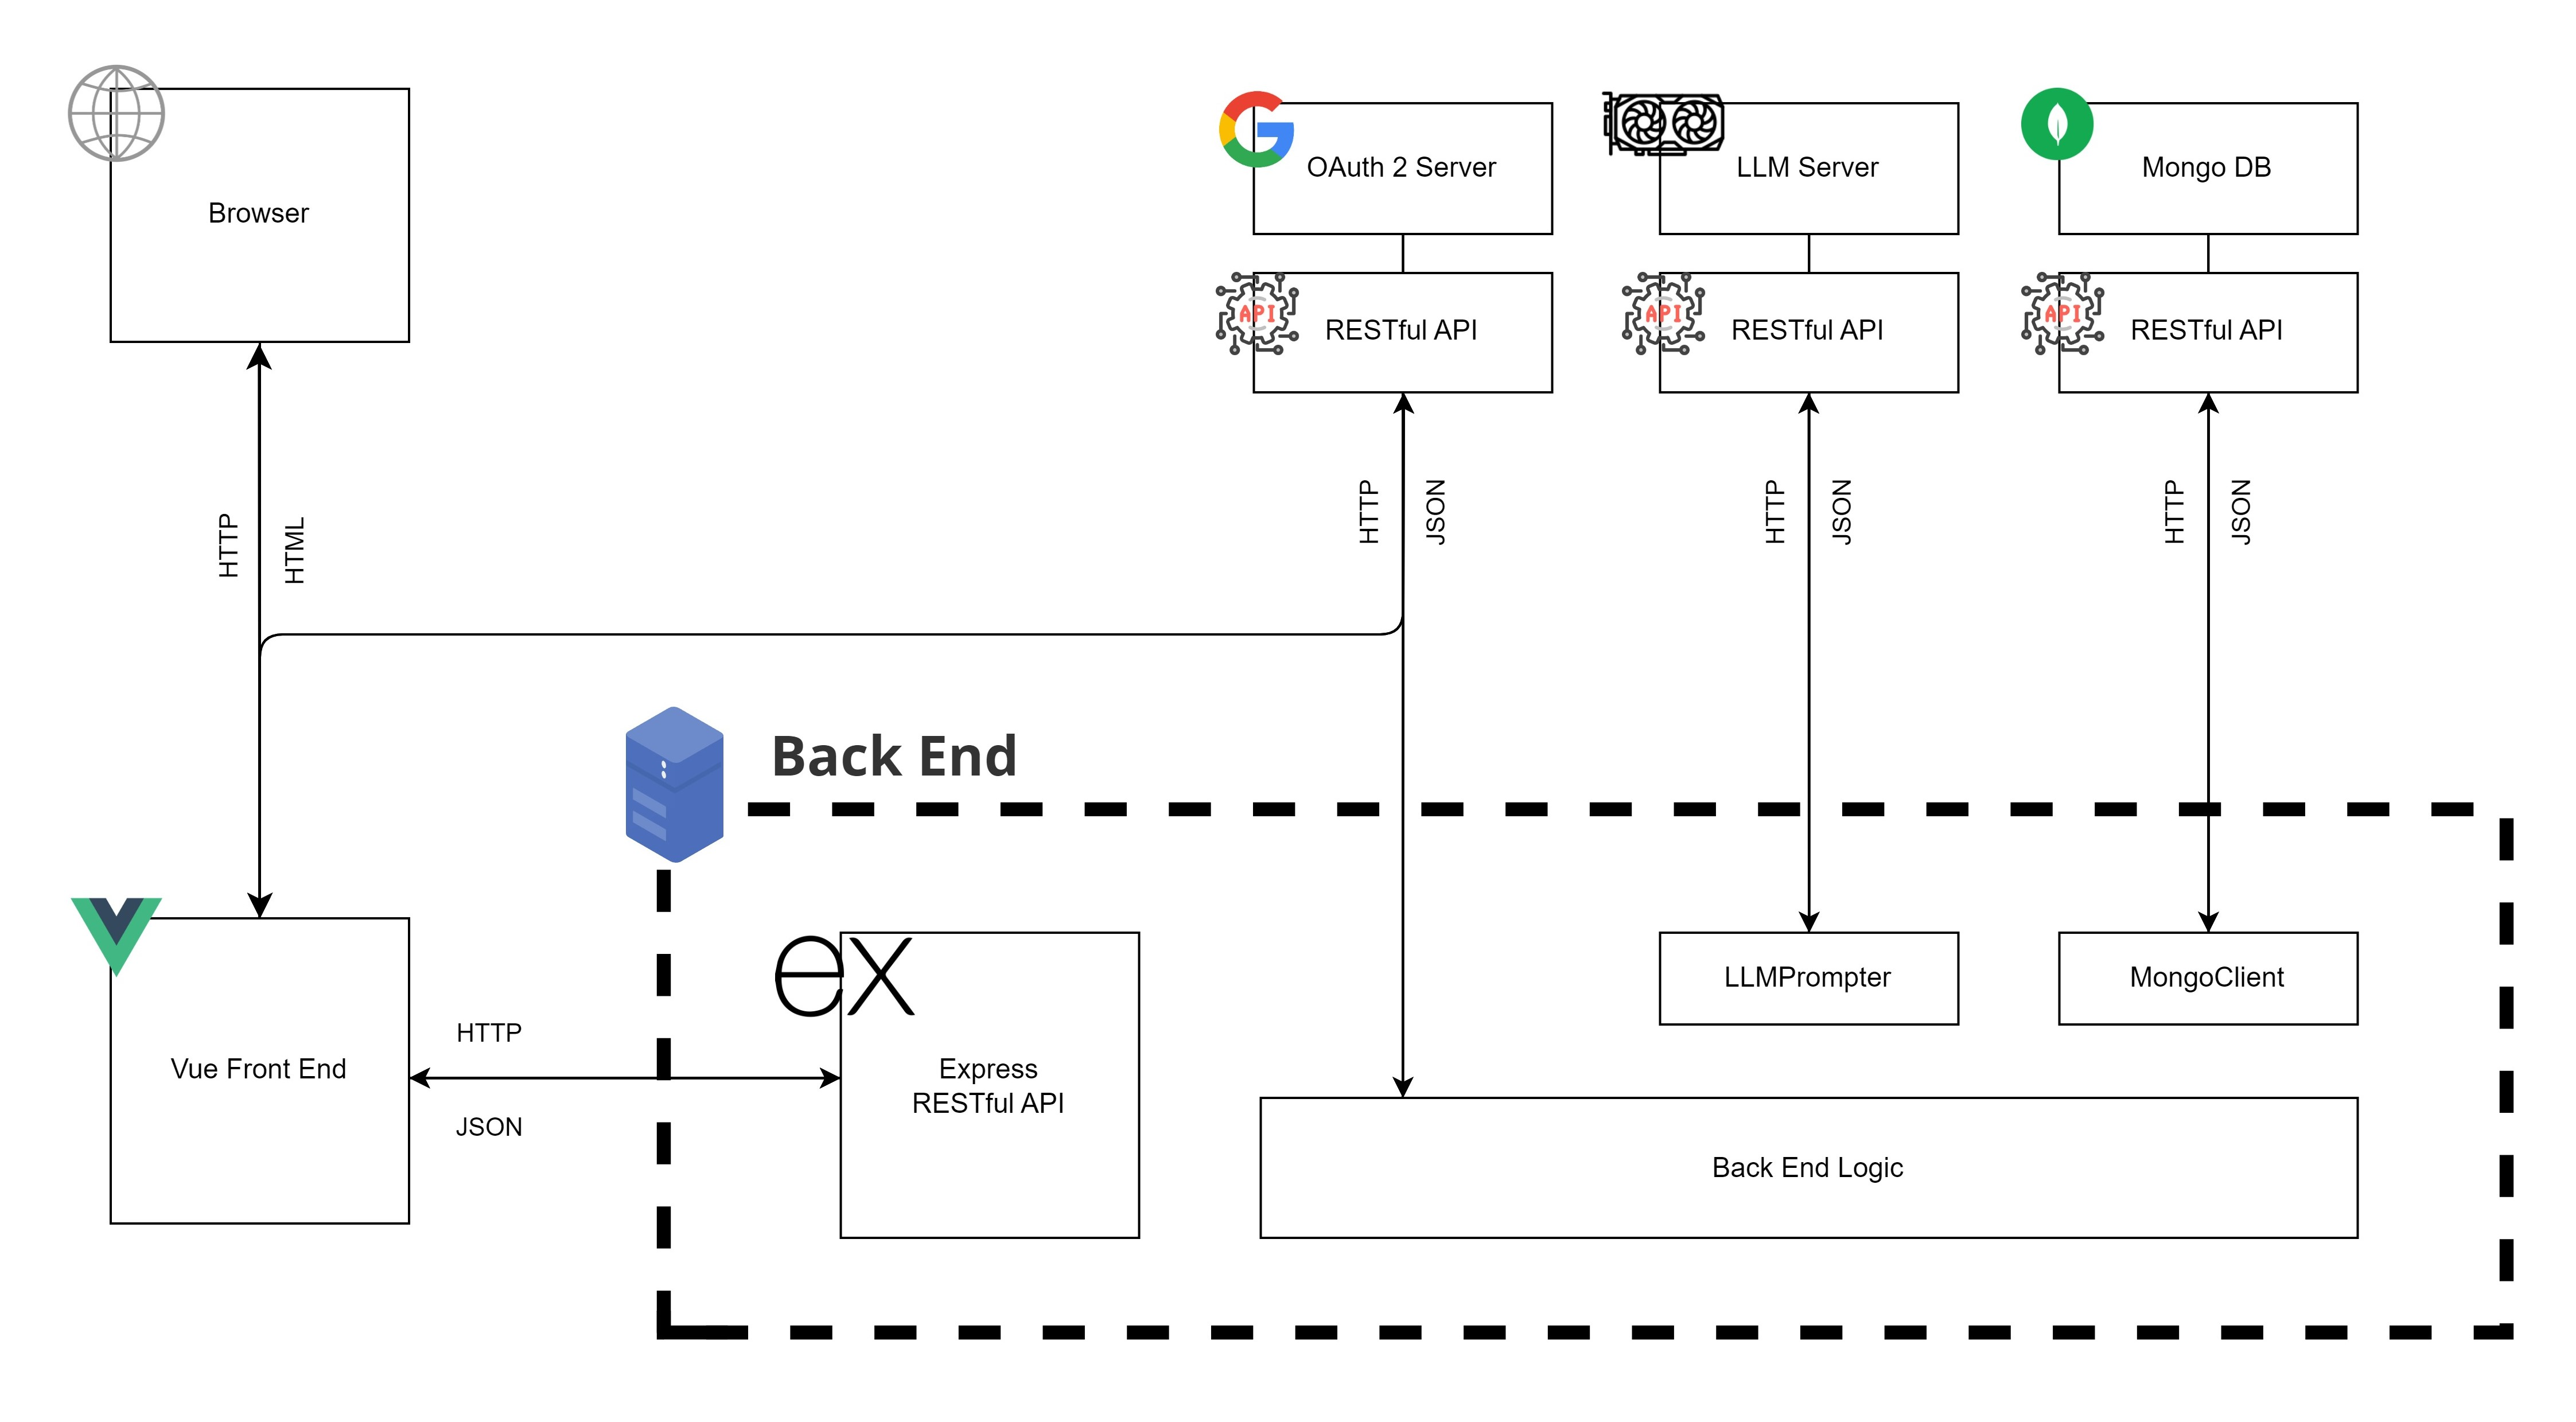
\includegraphics[width=0.95\textwidth]{images/architecture.jpg}
  \caption{\small The architecture diagram ot the MindMerge system}
\end{figure}
The architecture is relatively simple,
comprising two classical components: the front end and the back end, along with several smaller components (browser, OAuth server, LLM service, and MongoDB).
\newline \newline
The browser communicates with the front end using the HTTP protocol and HTML format.
\newline \newline
The front end, based on the Vue library, accesses resources provided by the back end using HTTP with JSON data format.
\newline \newline
Authentication is provided by a third-party OAuth server, that communicate with both the front end and back end via HTTP/JSON.
\newline \newline
The back end is the most complex component consists of several sub-components, including:
\begin{itemize}
  \item A part providing RESTful APIs based on Express.js
  \item A component dedicated to communicating with the database (MongoClient)
  \item A module for communicating with the LLM service (LLMPrompter)
  \item Logic containing all functions necessary for the application's operation.
\end{itemize}
All the communications that the backend has with the external world are made through HTTP with json format.

\section{Product Backlog}


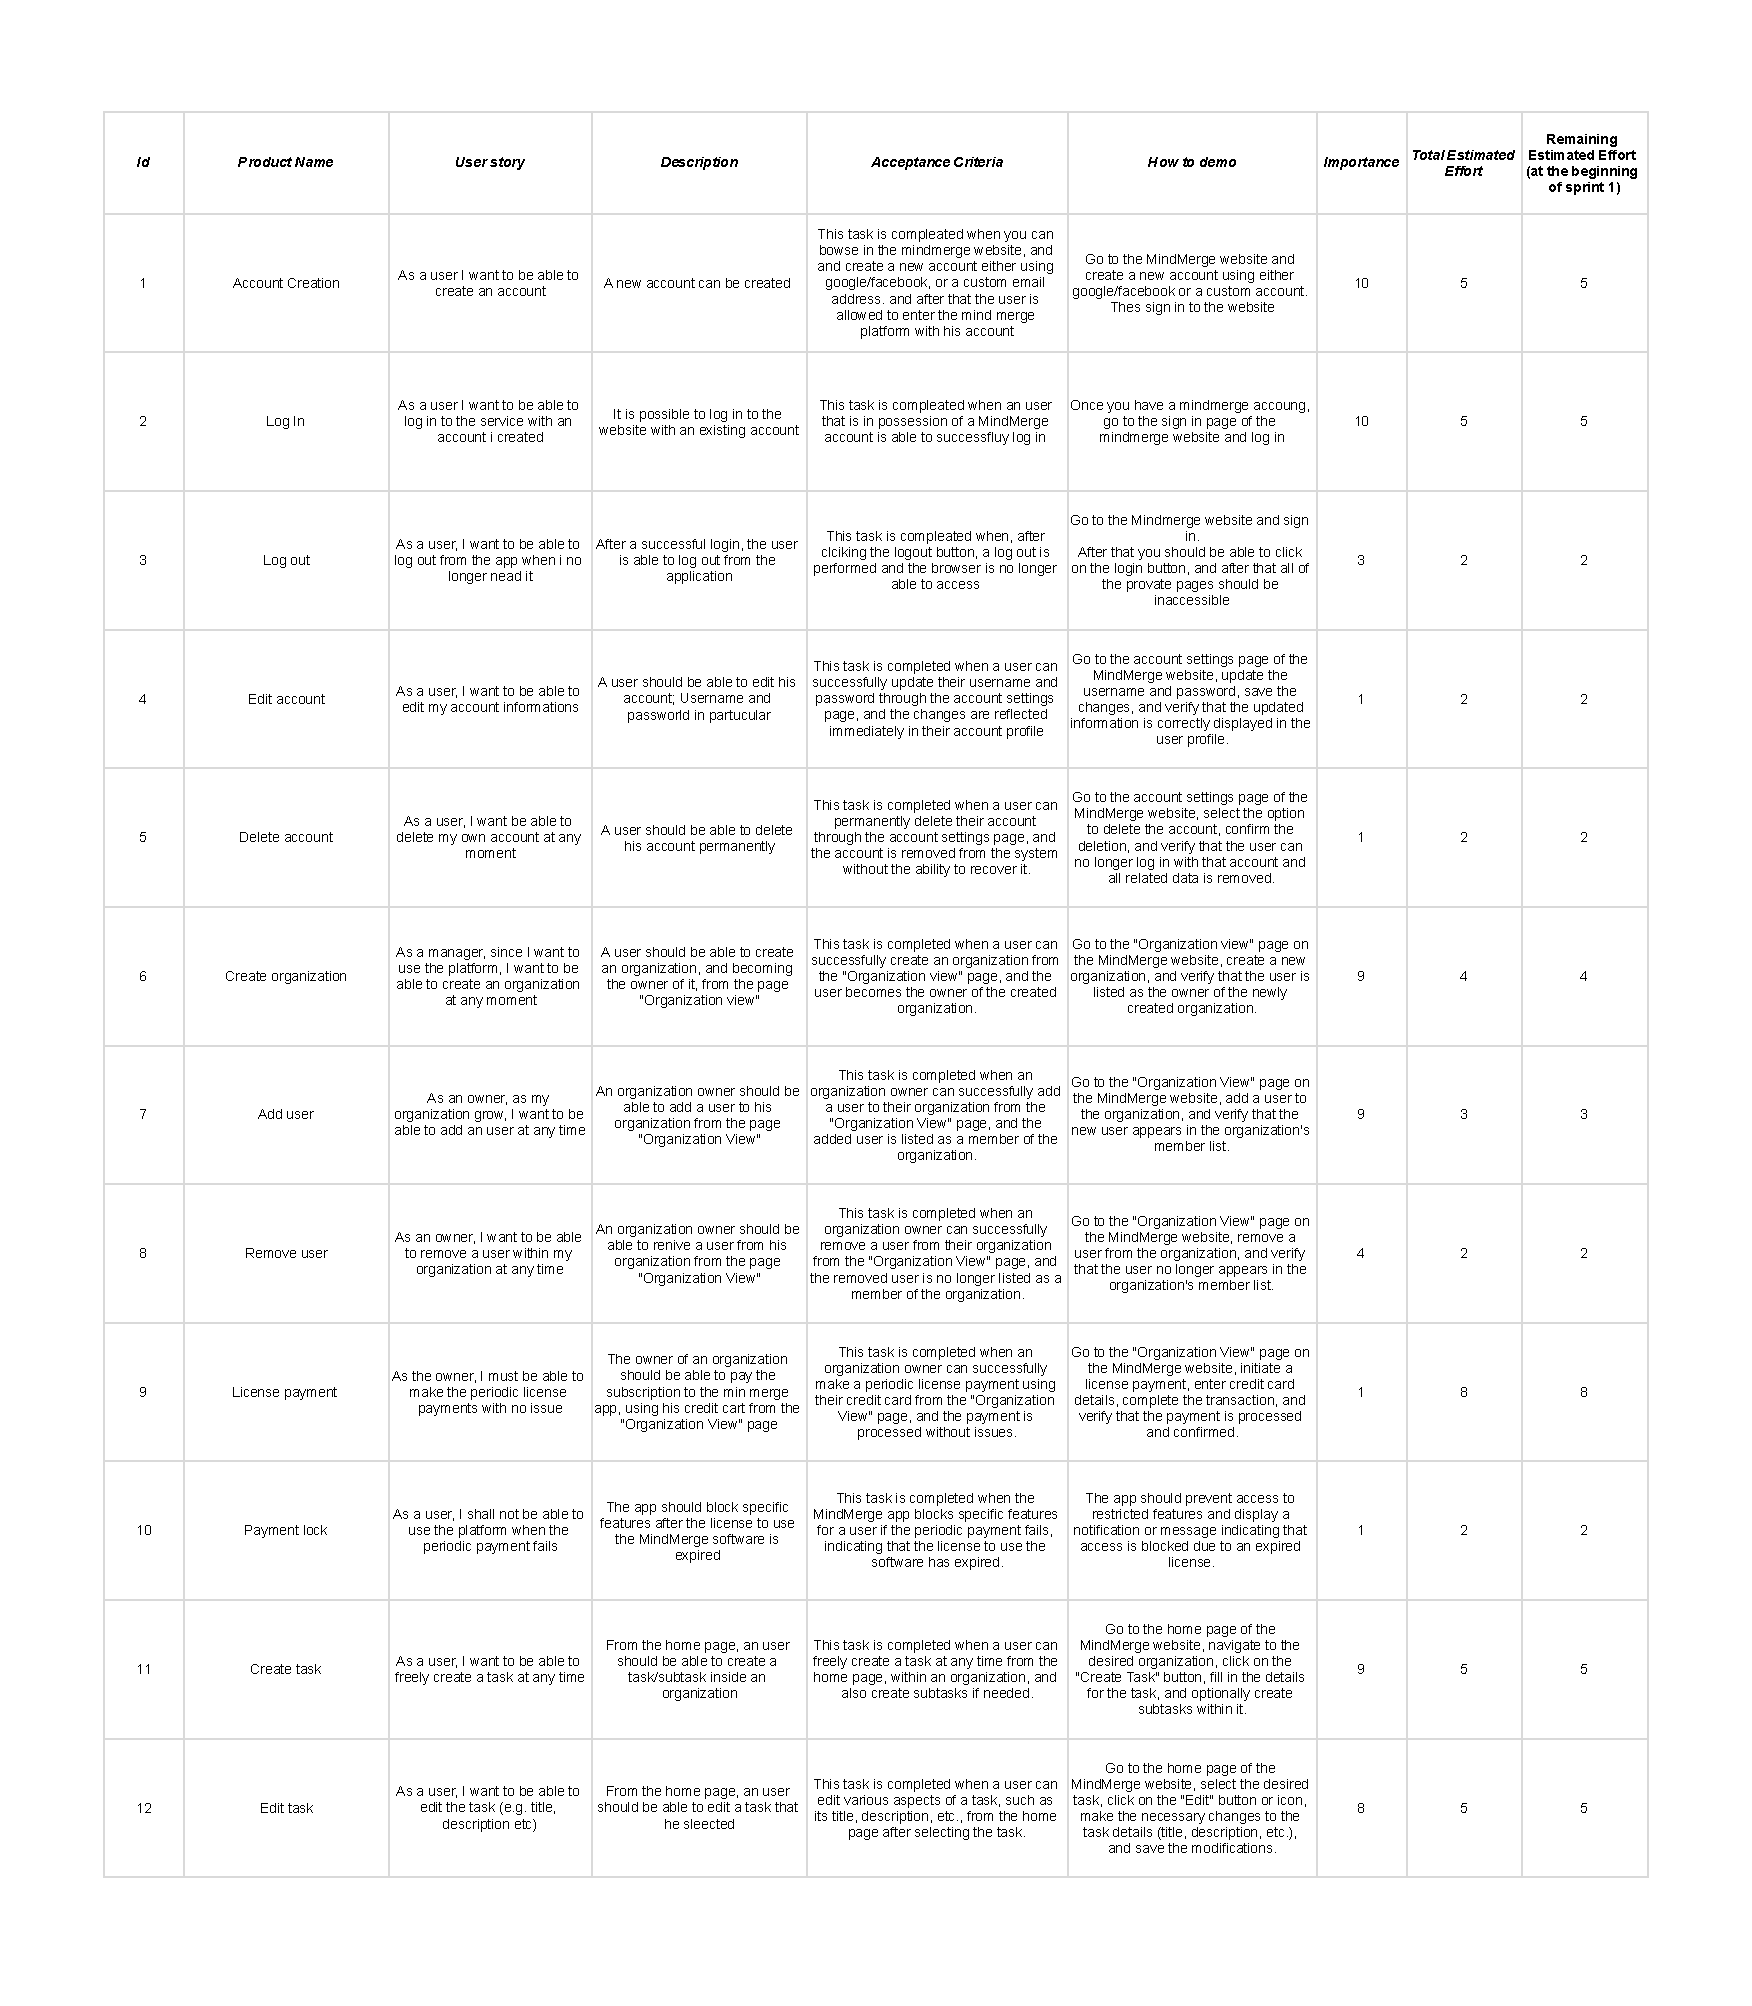
\includepdf[pages=-]{images/product_backlog.pdf} 

\section{Definition of Tests}

\subsection*{Test DatabaseManager:TaskManager}

This section contains the tests for the TaskManager class, which is responsible for managing tasks in the database.
\newline
\adjustbox{max width=\textwidth}{
  \begin{tabular}{|l|c|l|l|l|l|l|}
    \hline
    \multicolumn{1}{|c|}{\cellcolor[HTML]{FFFFFF}\textbf{Number}} & \cellcolor[HTML]{FFFFFF}\textbf{Test Group}                                  & \multicolumn{1}{c|}{\cellcolor[HTML]{FFFFFF}\textbf{Test Type}} & \multicolumn{1}{c|}{\textbf{Name}}             & \multicolumn{1}{c|}{\textbf{Test case data}}                                                                                     & \multicolumn{1}{c|}{\textbf{Preconditions}}                                                    & \multicolumn{1}{c|}{\textbf{Expected Results}}                                                                                \\ \hline
    \rowcolor[HTML]{FFFFFF}
    1                                                             & \cellcolor[HTML]{FFFFFF}                                                     & {\color[HTML]{11734B} Automated}                                & successul task creation                        & Call the method TaskManager.createTask three times with different task names and check the results.                              & The TaskModel collection is empty.                                                             & A new task is created each time with the expected attributes and status code. The tasks are correctly stored in the database. \\ \cline{1-1} \cline{3-7}
    \rowcolor[HTML]{FFFFFF}
    2                                                             & \cellcolor[HTML]{FFFFFF}                                                     & {\color[HTML]{11734B} Automated}                                & unsuccessul task creation                      & Call the method TaskManager.createTask with various invalid task data                                                            & The TaskModel collection is empty.                                                             & Errors.BAD\_REQUEST is returned                                                                                               \\ \cline{1-1} \cline{3-7}
    \rowcolor[HTML]{FFFFFF}
    3                                                             & \cellcolor[HTML]{FFFFFF}                                                     & {\color[HTML]{11734B} Automated}                                & successul task note creation                   & Call the method TaskManager.createTaskNotes and pass a valid taskId and notes                                                    & The TaskModel has a few tasks created where notes can be added                                 & Notes for tasks are created                                                                                                   \\ \cline{1-1} \cline{3-7}
    \rowcolor[HTML]{FFFFFF}
    4                                                             & \cellcolor[HTML]{FFFFFF}                                                     & {\color[HTML]{11734B} Automated}                                & unsuccessul task note creation                 & Call the method TaskManager.createTaskNotes with invalid parameters, and/or with non existing task                               & The TaskModel has a few tasks created where notes can be added                                 & Errors.NOT\_FOUND or Errors.BAD\_REQUEST is returned based on the invalid parameters                                          \\ \cline{1-1} \cline{3-7}
    \rowcolor[HTML]{FFFFFF}
    5                                                             & \cellcolor[HTML]{FFFFFF}                                                     & {\color[HTML]{11734B} Automated}                                & successful task report schedule creation       & Call TaskManager.createTaskReportSchedule with valid report schedule data                                                        & The TaskModel has a few tasks created where schedules can be added                             & A successful status code is returned and the task report schedules are created correctly.                                     \\ \cline{1-1} \cline{3-7}
    \rowcolor[HTML]{FFFFFF}
    6                                                             & \cellcolor[HTML]{FFFFFF}                                                     & {\color[HTML]{11734B} Automated}                                & unsuccessful task report schedule creation     & Call TaskManager.createTaskReportSchedule with invalid report schedule data                                                      & The TaskModel has a few tasks created where schedules can be added                             & Errors.NOT\_FOUND or Errors.BAD\_REQUEST is returned based on the invalid parameters                                          \\ \cline{1-1} \cline{3-7}
    \rowcolor[HTML]{FFFFFF}
    7                                                             & \cellcolor[HTML]{FFFFFF}                                                     & {\color[HTML]{11734B} Automated}                                & successful task update                         & Call the method TaskManager.updateTask and pass valid parameters                                                                 & The TaskModel has a few tasks created that can be edited for the test                          & Tasks are successfully updated with the correct data                                                                          \\ \cline{1-1} \cline{3-7}
    \rowcolor[HTML]{FFFFFF}
    8                                                             & \cellcolor[HTML]{FFFFFF}                                                     & {\color[HTML]{11734B} Automated}                                & unsuccessful task update                       & Call the method TaskManager.updateTask and pass non valid parameters                                                             & The TaskModel has a few tasks created that can be edited for the test                          & Errors.NOT\_FOUND or Errors.BAD\_REQUEST is returned based on the invalid parameters                                          \\ \cline{1-1} \cline{3-7}
    \rowcolor[HTML]{FFFFFF}
    9                                                             & \cellcolor[HTML]{FFFFFF}                                                     & {\color[HTML]{11734B} Automated}                                & successful update last task update             & Call TaskManager.updateTaskLastUpdated and pass the id of an existing task                                                       & The TaskModel has a few tasks created that can be edited for the test                          & The task's lastUpdated field is updated correctly, with the current time                                                      \\ \cline{1-1} \cline{3-7}
    \rowcolor[HTML]{FFFFFF}
    10                                                            & \cellcolor[HTML]{FFFFFF}                                                     & {\color[HTML]{11734B} Automated}                                & unsuccessful update last task update           & Call TaskManager.updateTaskLastUpdated and pass the id of a non existing task                                                    & The TaskModel has a few tasks created that can be edited for the test                          & The expected status code for each update attempt is Errors.NOT\_FOUND                                                         \\ \cline{1-1} \cline{3-7}
    \rowcolor[HTML]{FFFFFF}
    11                                                            & \cellcolor[HTML]{FFFFFF}                                                     & {\color[HTML]{11734B} Automated}                                & successful update task name                    & Call the method TaskManager.updateTaskName with valid task and organization IDs, and a new task name                             & The TaskModel has a few tasks created that can be edited for the test                          & The task's name is successfuly updated in the database                                                                        \\ \cline{1-1} \cline{3-7}
    \rowcolor[HTML]{FFFFFF}
    12                                                            & \cellcolor[HTML]{FFFFFF}                                                     & {\color[HTML]{11734B} Automated}                                & unsuccessful update task name                  & Call the method TaskManager.updateTaskName with invalid task and organization IDs, and/or an invalid name                        & The TaskModel has a few tasks created that can be edited for the test                          & Errors.NOT\_FOUND or Errors.BAD\_REQUEST is returned based on the invalid parameters                                          \\ \cline{1-1} \cline{3-7}
    \rowcolor[HTML]{FFFFFF}
    13                                                            & \cellcolor[HTML]{FFFFFF}                                                     & {\color[HTML]{11734B} Automated}                                & successful update task description             & Call the method TaskManager.updateTaskDescription with valid task data                                                           & The TaskModel has a few tasks created that can be edited for the test                          & The task's description is successfuly updated in the database                                                                 \\ \cline{1-1} \cline{3-7}
    \rowcolor[HTML]{FFFFFF}
    14                                                            & \cellcolor[HTML]{FFFFFF}                                                     & {\color[HTML]{11734B} Automated}                                & unsuccessful update task description           & Call the method TaskManager.updateTaskDescription with invalid task data                                                         & The TaskModel has a few tasks created that can be edited for the test                          & Errors.NOT\_FOUND or Errors.BAD\_REQUEST is returned based on the invalid parameters                                          \\ \cline{1-1} \cline{3-7}
    \cellcolor[HTML]{FFFFFF}15                                    & \cellcolor[HTML]{FFFFFF}                                                     & \cellcolor[HTML]{FFFFFF}{\color[HTML]{11734B} Automated}        & successful update task status                  & \cellcolor[HTML]{FFFFFF}Call the method TaskManager.updateTaskStatus with valid task and status                                  & \cellcolor[HTML]{FFFFFF}The TaskModel has a few tasks created that can be edited for the test  & \cellcolor[HTML]{FFFFFF}The task's status is successfuly updated in the database                                              \\ \cline{1-1} \cline{3-7}
    \cellcolor[HTML]{FFFFFF}16                                    & \cellcolor[HTML]{FFFFFF}                                                     & \cellcolor[HTML]{FFFFFF}{\color[HTML]{11734B} Automated}        & unsuccessful update task status                & \cellcolor[HTML]{FFFFFF}Call the method TaskManager.updateTaskStatus with invalid task ids and states id                         & \cellcolor[HTML]{FFFFFF}The TaskModel has a few tasks created that can be edited for the test  & \cellcolor[HTML]{FFFFFF}Errors.NOT\_FOUND or Errors.BAD\_REQUEST is returned based on the invalid parameters                  \\ \cline{1-1} \cline{3-7}
    \cellcolor[HTML]{FFFFFF}17                                    & \cellcolor[HTML]{FFFFFF}                                                     & \cellcolor[HTML]{FFFFFF}{\color[HTML]{11734B} Automated}        & successful update task notes                   & \cellcolor[HTML]{FFFFFF}Call the method TaskManager.updateTaskNotes with valid data                                              & \cellcolor[HTML]{FFFFFF}The TaskModel has a few tasks created that can be edited for the test  & \cellcolor[HTML]{FFFFFF}The task's notes are successfuly updated in the database                                              \\ \cline{1-1} \cline{3-7}
    \cellcolor[HTML]{FFFFFF}18                                    & \cellcolor[HTML]{FFFFFF}                                                     & \cellcolor[HTML]{FFFFFF}{\color[HTML]{11734B} Automated}        & unsuccessful update task notes                 & \cellcolor[HTML]{FFFFFF}Call the method TaskManager.updateTaskNotes with invalid data or task id                                 & \cellcolor[HTML]{FFFFFF}The TaskModel has a few tasks created that can be edited for the test  & \cellcolor[HTML]{FFFFFF}Errors.NOT\_FOUND or Errors.BAD\_REQUEST is returned based on the invalid parameters                  \\ \cline{1-1} \cline{3-7}
    \cellcolor[HTML]{FFFFFF}19                                    & \cellcolor[HTML]{FFFFFF}                                                     & \cellcolor[HTML]{FFFFFF}{\color[HTML]{11734B} Automated}        & successful add new assaignee                   & \cellcolor[HTML]{FFFFFF}Call the method TaskManager.addNewAssignee with valid assignee ID and task id                            & \cellcolor[HTML]{FFFFFF}The TaskModel has a few tasks created that can be edited for the test  & \cellcolor[HTML]{FFFFFF}The task's assainees list is successfuly updated in the database                                      \\ \cline{1-1} \cline{3-7}
    \cellcolor[HTML]{FFFFFF}20                                    & \cellcolor[HTML]{FFFFFF}                                                     & \cellcolor[HTML]{FFFFFF}{\color[HTML]{11734B} Automated}        & unsuccessful add new assaignee                 & \cellcolor[HTML]{FFFFFF}Call the method TaskManager.addNewAssignee with invalid assignee ID or task id                           & \cellcolor[HTML]{FFFFFF}The TaskModel has a few tasks created that can be edited for the test  & \cellcolor[HTML]{FFFFFF}Errors.NOT\_FOUND or Errors.BAD\_REQUEST is returned based on the invalid parameters                  \\ \cline{1-1} \cline{3-7}
    \cellcolor[HTML]{FFFFFF}21                                    & \cellcolor[HTML]{FFFFFF}                                                     & \cellcolor[HTML]{FFFFFF}{\color[HTML]{11734B} Automated}        & successful update task manager                 & \cellcolor[HTML]{FFFFFF}Call the method TaskManager.updateTaskManager with a valid new manager, and task id                      & \cellcolor[HTML]{FFFFFF}The TaskModel has a few tasks created that can be edited for the test  & \cellcolor[HTML]{FFFFFF}The task's manager is successfuly updated in the database                                             \\ \cline{1-1} \cline{3-7}
    \cellcolor[HTML]{FFFFFF}22                                    & \cellcolor[HTML]{FFFFFF}                                                     & \cellcolor[HTML]{FFFFFF}{\color[HTML]{11734B} Automated}        & unsuccessful update task manager               & \cellcolor[HTML]{FFFFFF}Call the method TaskManager.updateTaskManager with an invalid new manager, or task id                    & \cellcolor[HTML]{FFFFFF}The TaskModel has a few tasks created that can be edited for the test  & \cellcolor[HTML]{FFFFFF}Errors.NOT\_FOUND or Errors.BAD\_REQUEST is returned based on the invalid parameters                  \\ \cline{1-1} \cline{3-7}
    \cellcolor[HTML]{FFFFFF}23                                    & \cellcolor[HTML]{FFFFFF}                                                     & \cellcolor[HTML]{FFFFFF}{\color[HTML]{11734B} Automated}        & successful enable and disable notification     & \cellcolor[HTML]{FFFFFF}Call TaskManager.enableNotification and TaskManager.disableNotification with valid task IDs              & \cellcolor[HTML]{FFFFFF}The TaskModel has a few tasks created that can be edited for the test  & \cellcolor[HTML]{FFFFFF}The task's notification flag is successfuly updated in the database                                   \\ \cline{1-1} \cline{3-7}
    \cellcolor[HTML]{FFFFFF}24                                    & \cellcolor[HTML]{FFFFFF}                                                     & \cellcolor[HTML]{FFFFFF}{\color[HTML]{11734B} Automated}        & unsuccessful enable and disable notification   & \cellcolor[HTML]{FFFFFF}Call TaskManager.enableNotification and TaskManager.disableNotification with invalid task IDs            & \cellcolor[HTML]{FFFFFF}The TaskModel has a few tasks created that can be edited for the test  & \cellcolor[HTML]{FFFFFF}Errors.NOT\_FOUND or Errors.BAD\_REQUEST is returned based on the invalid parameters                  \\ \cline{1-1} \cline{3-7}
    \cellcolor[HTML]{FFFFFF}25                                    & \cellcolor[HTML]{FFFFFF}                                                     & \cellcolor[HTML]{FFFFFF}{\color[HTML]{11734B} Automated}        & successful add child task                      & \cellcolor[HTML]{FFFFFF}Call the method TaskManager.addChildTask with a valid task id and child task id                          & \cellcolor[HTML]{FFFFFF}The TaskModel has a few tasks created that can be edited for the test  & \cellcolor[HTML]{FFFFFF}The task's notes are successfuly updated in the database                                              \\ \cline{1-1} \cline{3-7}
    \cellcolor[HTML]{FFFFFF}26                                    & \cellcolor[HTML]{FFFFFF}                                                     & \cellcolor[HTML]{FFFFFF}{\color[HTML]{11734B} Automated}        & unsuccessful add child task                    & \cellcolor[HTML]{FFFFFF}Call the method TaskManager.addChildTask with an invalid task id or child task id                        & \cellcolor[HTML]{FFFFFF}The TaskModel has a few tasks created that can be edited for the test  & \cellcolor[HTML]{FFFFFF}Errors.NOT\_FOUND or Errors.BAD\_REQUEST is returned based on the invalid parameters                  \\ \cline{1-1} \cline{3-7}
    \cellcolor[HTML]{FFFFFF}27                                    & \cellcolor[HTML]{FFFFFF}                                                     & \cellcolor[HTML]{FFFFFF}{\color[HTML]{11734B} Automated}        & successful update recursive permission value   & \cellcolor[HTML]{FFFFFF}Call the method TaskManager.updateTaskRecursivePermissionsValue with valid task id and permission value  & \cellcolor[HTML]{FFFFFF}The TaskModel has a few tasks created that can be edited for the test  & \cellcolor[HTML]{FFFFFF}The task's recursive permission value issuccessfuly updated in the database                           \\ \cline{1-1} \cline{3-7}
    \cellcolor[HTML]{FFFFFF}28                                    & \cellcolor[HTML]{FFFFFF}                                                     & \cellcolor[HTML]{FFFFFF}{\color[HTML]{11734B} Automated}        & unsuccessful update recursive permission value & \cellcolor[HTML]{FFFFFF}Call the method TaskManager.updateTaskRecursivePermissionsValue with invalid task id or permission value & \cellcolor[HTML]{FFFFFF}The TaskModel has a few tasks created that can be edited for the test  & \cellcolor[HTML]{FFFFFF}Errors.NOT\_FOUND or Errors.BAD\_REQUEST is returned based on the invalid parameters                  \\ \cline{1-1} \cline{3-7}
    \rowcolor[HTML]{FFFFFF}
    29                                                            & \cellcolor[HTML]{FFFFFF}                                                     & {\color[HTML]{11734B} Automated}                                & successful delete task                         & Call the method TaskManager.deleteTask with valid taskId and organizationId                                                      & The TaskModel has a few tasks created that can be deleted for the test                         & the specified task is successfuly deleted in the database                                                                     \\ \cline{1-1} \cline{3-7}
    \rowcolor[HTML]{FFFFFF}
    30                                                            & \cellcolor[HTML]{FFFFFF}                                                     & {\color[HTML]{11734B} Automated}                                & unsuccessful delete task                       & Call the method TaskManager.deleteTask with invalid taskId or organizationId                                                     & The TaskModel has a few tasks created that can be deleted for the test                         & Errors.NOT\_FOUND or Errors.BAD\_REQUEST is returned based on the invalid parameters                                          \\ \cline{1-1} \cline{3-7}
    \cellcolor[HTML]{FFFFFF}31                                    & \cellcolor[HTML]{FFFFFF}                                                     & \cellcolor[HTML]{FFFFFF}{\color[HTML]{11734B} Automated}        & successful delete task notes                   & Call TaskModel.deleteTaskNote with a valid task and note id                                                                      & \cellcolor[HTML]{FFFFFF}The TaskModel has a few tasks created that can be deleted for the test & \cellcolor[HTML]{FFFFFF}the specified task note is successfuly deleted in the database                                        \\ \cline{1-1} \cline{3-7}
    \cellcolor[HTML]{FFFFFF}32                                    & \cellcolor[HTML]{FFFFFF}                                                     & \cellcolor[HTML]{FFFFFF}{\color[HTML]{11734B} Automated}        & unsuccessful delete task notes                 & Call TaskModel.deleteTaskNote with an invalid task or note id                                                                    & \cellcolor[HTML]{FFFFFF}The TaskModel has a few tasks created that can be deleted for the test & \cellcolor[HTML]{FFFFFF}Errors.NOT\_FOUND or Errors.BAD\_REQUEST is returned based on the invalid parameters                  \\ \cline{1-1} \cline{3-7}
    \cellcolor[HTML]{FFFFFF}33                                    & \cellcolor[HTML]{FFFFFF}                                                     & \cellcolor[HTML]{FFFFFF}{\color[HTML]{11734B} Automated}        & successful delete task assignee                & Call the method TaskManager.deleteTaskAssignee with valid task id, user id, and assignee id                                      & \cellcolor[HTML]{FFFFFF}The TaskModel has a few tasks created that can be deleted for the test & \cellcolor[HTML]{FFFFFF}the specified task assignee is successfuly deleted  from the assignees list in the database           \\ \cline{1-1} \cline{3-7}
    \cellcolor[HTML]{FFFFFF}34                                    & \cellcolor[HTML]{FFFFFF}                                                     & \cellcolor[HTML]{FFFFFF}{\color[HTML]{11734B} Automated}        & usuccessful delete task assignee               & Delete task assignee with invalid task id, assignee id, or organization id                                                       & \cellcolor[HTML]{FFFFFF}The TaskModel has a few tasks created that can be deleted for the test & \cellcolor[HTML]{FFFFFF}Errors.NOT\_FOUND or Errors.BAD\_REQUEST is returned based on the invalid parameters                  \\ \cline{1-1} \cline{3-7}
    \cellcolor[HTML]{FFFFFF}35                                    & \cellcolor[HTML]{FFFFFF}                                                     & \cellcolor[HTML]{FFFFFF}{\color[HTML]{11734B} Automated}        & successful delete report schedule              & \cellcolor[HTML]{FFFFFF}Delete report schedule with valid task id, report schedule id, and organization id                       & \cellcolor[HTML]{FFFFFF}The TaskModel has a few tasks created that can be deleted for the test & \cellcolor[HTML]{FFFFFF}the specified task report schedule is successfuly deleted in the database                             \\ \cline{1-1} \cline{3-7}
    \cellcolor[HTML]{FFFFFF}36                                    & \cellcolor[HTML]{FFFFFF}                                                     & \cellcolor[HTML]{FFFFFF}{\color[HTML]{11734B} Automated}        & unsuccessful delete report schedule            & \cellcolor[HTML]{FFFFFF}Delete report schedule with invalid task id, report schedule id, or organization id                      & \cellcolor[HTML]{FFFFFF}The TaskModel has a few tasks created that can be deleted for the test & \cellcolor[HTML]{FFFFFF}Errors.NOT\_FOUND or Errors.BAD\_REQUEST is returned based on the invalid parameters                  \\ \cline{1-1} \cline{3-7}
    \cellcolor[HTML]{FFFFFF}37                                    & \cellcolor[HTML]{FFFFFF}                                                     & \cellcolor[HTML]{FFFFFF}{\color[HTML]{11734B} Automated}        & successful remove child task                   & \cellcolor[HTML]{FFFFFF}Remove child task with valid parent task id, child task id, and organization id                          & \cellcolor[HTML]{FFFFFF}The TaskModel has a few tasks created that can be deleted for the test & \cellcolor[HTML]{FFFFFF}the specified child task is successfuly deleted  from the child tasks list in the database            \\ \cline{1-1} \cline{3-7}
    \cellcolor[HTML]{FFFFFF}38                                    & \cellcolor[HTML]{FFFFFF}                                                     & \cellcolor[HTML]{FFFFFF}{\color[HTML]{11734B} Automated}        & unsuccessful remove child task                 & \cellcolor[HTML]{FFFFFF}Remove child task with invalid parent task id, child task id, or organization id                         & \cellcolor[HTML]{FFFFFF}The TaskModel has a few tasks created that can be deleted for the test & \cellcolor[HTML]{FFFFFF}Errors.NOT\_FOUND or Errors.BAD\_REQUEST is returned based on the invalid parameters                  \\ \cline{1-1} \cline{3-7}
    \cellcolor[HTML]{FFFFFF}39                                    & \cellcolor[HTML]{FFFFFF}                                                     & \cellcolor[HTML]{FFFFFF}{\color[HTML]{11734B} Automated}        & successful get task                            & \cellcolor[HTML]{FFFFFF}Get task with valid task id and organization id                                                          & \cellcolor[HTML]{FFFFFF}The TaskModel has a few tasks created that can be red for the test     & Successfully retrieve task details, returning Errors.OK                                                                       \\ \cline{1-1} \cline{3-7}
    \cellcolor[HTML]{FFFFFF}40                                    & \multirow{-40}{*}{\cellcolor[HTML]{FFFFFF}Test DatabaseManager::TaskManager} & \cellcolor[HTML]{FFFFFF}{\color[HTML]{11734B} Automated}        & unsuccessful get task                          & \cellcolor[HTML]{FFFFFF}Get task with invalid task id or organization id                                                         & \cellcolor[HTML]{FFFFFF}The TaskModel has a few tasks created that can be red for the test     & Task not found, returning Errors.NOT\_FOUND                                                                                   \\ \hline
  \end{tabular}
}

\subsection*{Test OrganizationManager}
This section is dedicated to the tests for the OrganizationManager class, which is responsible for managing organizations in the database.
\newline
\adjustbox{max width=\textwidth}{
  \begin{tabular}{|
      >{\columncolor[HTML]{FFFFFF}}l |
      >{\columncolor[HTML]{FFFFFF}}c |
      >{\columncolor[HTML]{FFFFFF}}l |l|l|l|l|}
    \hline
    41 & \cellcolor[HTML]{FFFFFF}                                            & {\color[HTML]{11734B} Automated} & test successfull add user to organization API       & Call the API to add an user to the organization with a valid requeat                           & User and Organizations are already present in the database                                                                               & The api returns OK (200) and the database is updated                                                                 \\ \cline{1-1} \cline{3-7}
    42 & \cellcolor[HTML]{FFFFFF}                                            & {\color[HTML]{11734B} Automated} & test unsuccesfull add user to organization API      & Call the API to add an user to the organization with invalid users/organizations               & User and Organizations are already present in the database                                                                               & \cellcolor[HTML]{FFFFFF}Not found error (404) or Bad request error (400) is returned based on the invalid parameters \\ \cline{1-1} \cline{3-7}
    43 & \cellcolor[HTML]{FFFFFF}                                            & {\color[HTML]{11734B} Automated} & test unautorized add user to organization API       & Call the API to add an user to the organization with invalid/missing autorization token        & User and Organizations are already present in the database                                                                               & Non autorized error (403)                                                                                            \\ \cline{1-1} \cline{3-7}
    44 & \cellcolor[HTML]{FFFFFF}                                            & {\color[HTML]{11734B} Automated} & test successfull remove user from organization API  & Call the API to remove an user from an organization with a valid requeat                       & User and Organizations are already present in the database                                                                               & The api returns OK (200) and the database is updated                                                                 \\ \cline{1-1} \cline{3-7}
    45 & \cellcolor[HTML]{FFFFFF}                                            & {\color[HTML]{11734B} Automated} & test unsuccesfull remove user from organization API & Call the API to remove an user from an organization with invalid users/organizations           & User and Organizations are already present in the database                                                                               & \cellcolor[HTML]{FFFFFF}Not found error (404) or Bad request error (400) is returned based on the invalid parameters \\ \cline{1-1} \cline{3-7}
    46 & \cellcolor[HTML]{FFFFFF}                                            & {\color[HTML]{11734B} Automated} & test unautorized remove user from organization API  & Call the API to remove an user from an organization with invalid/missing autorization token    & User and Organizations are already present in the database                                                                               & Non autorized error (403)                                                                                            \\ \cline{1-1} \cline{3-7}
    47 & \cellcolor[HTML]{FFFFFF}                                            & {\color[HTML]{11734B} Automated} & test successful calculate subscription price        & Call the method OrganizationManager.calculateSubscriptionPrice with a valid organization id    & an Organization with some users and soem tasks is present in the database                                                                & The function successfuly caluclate the price the ortanization should pay based on usage                              \\ \cline{1-1} \cline{3-7}
    48 & \cellcolor[HTML]{FFFFFF}                                            & {\color[HTML]{11734B} Automated} & test unsuccessful calculate subscription price      & Call the method OrganizationManager.calculateSubscriptionPrice with an invalid organization id & an Organization with some users and soem tasks is present in the database                                                                & Errors.NOT\_FOUND or Errors.BAD\_REQUEST is returned based on the invalid parameters                                 \\ \cline{1-1} \cline{3-7}
    49 & \cellcolor[HTML]{FFFFFF}                                            & {\color[HTML]{11734B} Automated} & test succesful verify subscription                  & Call the method OrganizationManager.verifySubscription with a valid organization id            & an Organization is present in the database                                                                                               & The function verify the current status of the organization subscription and returns it                               \\ \cline{1-1} \cline{3-7}
    50 & \cellcolor[HTML]{FFFFFF}                                            & {\color[HTML]{11734B} Automated} & test unsuccesful verify subscription                & Call the method OrganizationManager.verifySubscription with an invalid organization id         & an Organization is present in the database                                                                                               & Errors.NOT\_FOUND or Errors.BAD\_REQUEST is returned based on the invalid parameters                                 \\ \cline{1-1} \cline{3-7}
    51 & \cellcolor[HTML]{FFFFFF}                                            & {\color[HTML]{11734B} Automated} & test successful pay subscription                    & Call the API to pay the subscription with valid organization, and credit card informations     & an Organization is present in the database, A connection with a bancking service has been established, A valid tast credit card is ready & \cellcolor[HTML]{FFFFFF}The payment is successful                                                                    \\ \cline{1-1} \cline{3-7}
    52 & \multirow{-12}{*}{\cellcolor[HTML]{FFFFFF}Test OrganizationManager} & {\color[HTML]{11734B} Automated} & test unsuccessful pay subscription                  & Call the API to pay the subscription with invalid organization, or credit card informations    & an Organization is present in the database, A connection with a bancking service has been established, A valid tast credit card is ready & The payment is not successful                                                                                        \\ \hline
  \end{tabular}
}

\subsection*{Test Report Page}
This section includes manual tests for the Report Page, which is responsible for generating reports.
\newline
\adjustbox{max width=\textwidth}{
  \begin{tabular}{|
      >{\columncolor[HTML]{FFFFFF}}l |
      >{\columncolor[HTML]{FFFFFF}}c |
      >{\columncolor[HTML]{FFFFFF}}l |l|l|l|l|}
    \hline
    53 & \cellcolor[HTML]{FFFFFF}                                   & {\color[HTML]{473821} Manual} & test add periodic report    & Go to the report page and take a look at the list of scheduled reports. Then add a few new repors by using the button "Add report schedule" & The backend, the front end and the database are running. You have access to a testing account & The added report are displayed in the table and all the informations are corrects. This is true even after a log out and a browser cash refresh                                            \\ \cline{1-1} \cline{3-7}
    54 & \multirow{-2}{*}{\cellcolor[HTML]{FFFFFF}Test Report Page} & {\color[HTML]{473821} Manual} & test delete periodic report & Go to the report page and take a look at the list of scheduled reports. Then click the delete button on some of them.                       & The backend, the front end and the database are running. You have access to a testing account & The deleted reports are no longer displayed in the list This is true even after a log out and a browser cash refresh. The user no longer receive notifications about the scheduler reports \\ \hline
  \end{tabular}
}
\subsection*{Test NotificationManager}
This section includes automated tests for the NotificationManager class, which is responsible for managing notifications in the database.
\newline
\adjustbox{max width=\textwidth}{
  \begin{tabular}{|
      >{\columncolor[HTML]{FFFFFF}}l |
      >{\columncolor[HTML]{FFFFFF}}c |
      >{\columncolor[HTML]{FFFFFF}}l |l|l|l|l|}
    \hline
    55 & \cellcolor[HTML]{FFFFFF}                                            & {\color[HTML]{11734B} Automated} & test successfull send notification           & Call method NotificationManager.sendNotification with valid parameters                                                     & At least one user and one notification are present in the database                                                                  & The notification is sent successfully                                                \\ \cline{1-1} \cline{3-7}
    56 & \cellcolor[HTML]{FFFFFF}                                            & {\color[HTML]{11734B} Automated} & test unsuccessfull send notification         & Call method NotificationManager.sendNotification with invalid parameters                                                   & At least one user and one notification are present in the database                                                                  & Errors.NOT\_FOUND or Errors.BAD\_REQUEST is returned based on the invalid parameters \\ \cline{1-1} \cline{3-7}
    57 & \cellcolor[HTML]{FFFFFF}                                            & {\color[HTML]{11734B} Automated} & test successfull send notification           & Call method ExternalNotificationManager.sendNotification with valid parameters                                             & At least one user and one notification are present in the database, we have a mail account with api access to test the notification & The notification is sent successfully                                                \\ \cline{1-1} \cline{3-7}
    58 & \cellcolor[HTML]{FFFFFF}                                            & {\color[HTML]{11734B} Automated} & test unsuccessfull send notification         & Call method ExternalNotificationManager.sendNotification with invalid parameters                                           & At least one user and one notification are present in the database, we have a mail account with api access to test the notification & Errors.NOT\_FOUND or Errors.BAD\_REQUEST is returned based on the invalid parameters \\ \cline{1-1} \cline{3-7}
    59 & \cellcolor[HTML]{FFFFFF}                                            & {\color[HTML]{11734B} Automated} & test successfull delete notification         & Call method InternalNotificationManager.deleteNotification with valid parameters (userId, notificationId, userToken)       & At least one user and one notification are present in the database                                                                  & The notification is deleted successfully                                             \\ \cline{1-1} \cline{3-7}
    60 & \cellcolor[HTML]{FFFFFF}                                            & {\color[HTML]{11734B} Automated} & test unsuccessfull delete notification       & Call method InternalNotificationManager.deleteNotification with invalid parameters (userId, notificationId, userToken)     & At least one user and one notification are present in the database                                                                  & Errors.NOT\_FOUND or Errors.BAD\_REQUEST is returned based on the invalid parameters \\ \cline{1-1} \cline{3-7}
    61 & \cellcolor[HTML]{FFFFFF}                                            & {\color[HTML]{11734B} Automated} & test successfull mark notification as read   & Call method InternalNotificationManager.markNotificationAsRead with valid parameters (userId, notificationId, userToken)   & At least one user and one notification are present in the database                                                                  & The notification gets marked as read                                                 \\ \cline{1-1} \cline{3-7}
    62 & \cellcolor[HTML]{FFFFFF}                                            & {\color[HTML]{11734B} Automated} & test unsuccessfull mark notification as read & Call method InternalNotificationManager.markNotificationAsRead with invalid parameters (userId, notificationId, userToken) & At least one user and one notification are present in the database                                                                  & Errors.NOT\_FOUND or Errors.BAD\_REQUEST is returned based on the invalid parameters \\ \cline{1-1} \cline{3-7}
    63 & \cellcolor[HTML]{FFFFFF}                                            & {\color[HTML]{11734B} Automated} & test successfull get notification details    & Call method InternalNotificationManager.getNotificationDetails with valid parameters (userId, notificationId, userToken)   & At least one user and one notification are present in the database                                                                  & A notification object is returned                                                    \\ \cline{1-1} \cline{3-7}
    64 & \cellcolor[HTML]{FFFFFF}                                            & {\color[HTML]{11734B} Automated} & test unsuccessfull get notification details  & Call method InternalNotificationManager.getNotificationDetails with invalid parameters (userId, notificationId, userToken) & At least one user and one notification are present in the database                                                                  & Errors.NOT\_FOUND or Errors.BAD\_REQUEST is returned based on the invalid parameters \\ \cline{1-1} \cline{3-7}
    65 & \cellcolor[HTML]{FFFFFF}                                            & {\color[HTML]{11734B} Automated} & test successfull get notification list       & Call method InternalNotificationManager.getNotificationDetails with valid parameters (userId, userToken)                   & At least one user is present in the database                                                                                        & The list of notifications linked to the userId are returned                          \\ \cline{1-1} \cline{3-7}
    66 & \multirow{-12}{*}{\cellcolor[HTML]{FFFFFF}Test NotificationManager} & {\color[HTML]{11734B} Automated} & test unsuccessfull get notification list     & Call method InternalNotificationManager.getNotificationDetails with invalid parameters (userId, userToken)                 & At least one user is present in the database                                                                                        & Errors.BAD\_REQUEST is returned                                                      \\ \hline
  \end{tabular}
}
\subsection*{Test ReportManager}
This section includes automated tests for the ReportManager class, which is responsible for managing reports in the database.
\newline
\adjustbox{max width=\textwidth}{
  \begin{tabular}{|
    >{\columncolor[HTML]{FFFFFF}}l |
    >{\columncolor[HTML]{FFFFFF}}c |
    >{\columncolor[HTML]{FFFFFF}}l |l|l|l|l|}
    \hline
    \textbf{67} & \cellcolor[HTML]{FFFFFF}                                      & {\color[HTML]{11734B} Automated} & test successfull set new report schedule                & Call method reportScheduler.scheduleReport with valid parameters (organizationId, taskId, reportPrompt, reportKind, reportFrequency, userId, userToken)   & Organization, Task, and User are already present in the database                                   & A new report schedule is set for said task and with said frequency                   \\ \cline{1-1} \cline{3-7} 
    68          & \cellcolor[HTML]{FFFFFF}                                      & {\color[HTML]{11734B} Automated} & test unsuccessfull set new report schedule              & Call method reportScheduler.scheduleReport with invalid parameters (organizationId, taskId, reportPrompt, reportKind, reportFrequency, userId, userToken) & Organization, Task, and User are already present in the database                                   & Errors.NOT\_FOUND or Errors.BAD\_REQUEST is returned based on the invalid parameters \\ \cline{1-1} \cline{3-7} 
    69          & \cellcolor[HTML]{FFFFFF}                                      & {\color[HTML]{11734B} Automated} & test successfull get report schedules                   & Call method reportScheduler.getReportSchedules with valid parameters (organizationId, taskId, userId, userToken)                                          & Organization, Task, and User are already present in the database                                   & The list of report schedules set for the task are returned                           \\ \cline{1-1} \cline{3-7} 
    70          & \cellcolor[HTML]{FFFFFF}                                      & {\color[HTML]{11734B} Automated} & test unsuccessfull get report schedules                 & Call method reportScheduler.getReportSchedules with invalid parameters (organizationId, taskId, userId, userToken)                                        & Organization, Task, and User are already present in the database                                   & Errors.NOT\_FOUND or Errors.BAD\_REQUEST is returned based on the invalid parameters \\ \cline{1-1} \cline{3-7} 
    71          & \cellcolor[HTML]{FFFFFF}                                      & {\color[HTML]{11734B} Automated} & test successfull remove report schedule                 & Call method reportScheduler.deleteReportSchedule with valid parameters (organizationId, taskId, reportId, userId, userToken)                              & Organization, Task, User and report are already present in the database                            & The report schedule gets deleted successfully                                        \\ \cline{1-1} \cline{3-7} 
    72          & \cellcolor[HTML]{FFFFFF}                                      & {\color[HTML]{11734B} Automated} & test unsuccessfull remove report schedule               & Call method reportScheduler.deleteReportSchedule with invalid parameters (organizationId, taskId, reportId, userId, userToken)                            & Organization, Task, User and report are already present in the database                            & Errors.NOT\_FOUND or Errors.BAD\_REQUEST is returned based on the invalid parameters \\ \cline{1-1} \cline{3-7} 
    73          & \cellcolor[HTML]{FFFFFF}                                      & {\color[HTML]{11734B} Automated} & test execute all pending periodic reports               & \cellcolor[HTML]{FFFFFF}Call method reportScheduler.executeScheduledReport with valid parameters (organizationId)                                         & An Organization is present in the database                                                         & All the pending reports gets executed                                                \\ \cline{1-1} \cline{3-7} 
    74          & \cellcolor[HTML]{FFFFFF}                                      & {\color[HTML]{11734B} Automated} & test unsuccessfull execute all pending periodic reports & \cellcolor[HTML]{FFFFFF}Call method reportScheduler.executeScheduledReport with invalid parameters (organizationId)                                       & An Organization is present in the database                                                         & Errors.BAD\_REQUEST is returned                                                      \\ \cline{1-1} \cline{3-7} 
    75          & \cellcolor[HTML]{FFFFFF}                                      & {\color[HTML]{11734B} Automated} & test successfull generate automatic report              & Call method AutomaticReportManager.generateAutomaticReports with valid parameters (organizationId, taskId, reportPrompt)                                  & Organization and Task are already present in the database, connection with LLM APIs is valid       & The report gets generated successfully                                               \\ \cline{1-1} \cline{3-7} 
    76          & \cellcolor[HTML]{FFFFFF}                                      & {\color[HTML]{11734B} Automated} & test unsuccessfull generate automatic report            & Call method AutomaticReportManager.generateAutomaticReports with invalid parameters (organizationId, taskId, reportPrompt)                                & Organization and Task are already present in the database, connection with LLM APIs is valid       & Errors.NOT\_FOUND or Errors.BAD\_REQUEST is returned based on the invalid parameters \\ \cline{1-1} \cline{3-7} 
    77          & \cellcolor[HTML]{FFFFFF}                                      & {\color[HTML]{11734B} Automated} & test successfull generate manual report                 & Call method ManualReportManager.generateManualReports with valid parameters (organizationId, taskId, reportPrompt)                                        & Organization and Task are already present in the database                                          & \cellcolor[HTML]{FFFFFF}The report gets generated successfully                       \\ \cline{1-1} \cline{3-7} 
    78          & \cellcolor[HTML]{FFFFFF}                                      & {\color[HTML]{11734B} Automated} & test unsuccessfull generate manual report               & Call method ManualReportManager.generateManualReports with invalid parameters (organizationId, taskId, reportPrompt)                                      & Organization and Task are already present in the database                                          & Errors.NOT\_FOUND or Errors.BAD\_REQUEST is returned based on the invalid parameters \\ \cline{1-1} \cline{3-7} 
    79          & \cellcolor[HTML]{FFFFFF}                                      & {\color[HTML]{11734B} Automated} & test successfull generate report                        & Call method ReportManager.generateReport with valid parameters (organizationId, taskId, reportPrompt, reportKind, userId, userToken)                      & Organization, Task and User are already present in the database, connection with LLM APIs is valid & The report gets generated successfully                                               \\ \cline{1-1} \cline{3-7} 
    80          & \multirow{-14}{*}{\cellcolor[HTML]{FFFFFF}Test ReportManager} & {\color[HTML]{11734B} Automated} & test unsuccessfull generate report                      & Call method ReportManager.generateReport with invalid parameters (organizationId, taskId, reportPrompt, reportKind, userId, userToken)                    & Organization, Task and User are already present in the database, connection with LLM APIs is valid & Errors.NOT\_FOUND or Errors.BAD\_REQUEST is returned based on the invalid parameters \\ \hline
    \end{tabular}
}

\section{Git Strategy}

We have chosen GitHub Flow as our Git strategy.
We chose it because is one of the simplest strategies and it is suitable for small teams.

\section{Definition Of Done}

\section{Sprint 1}

\subsection{Sprint 1 Backlog}
  \includegraphics[width=0.95\textwidth]{images/sprint_backlog.jpg}

\subsection{Sprint 1 Review and Retrospective}

\subsection{Burndown Chart}
  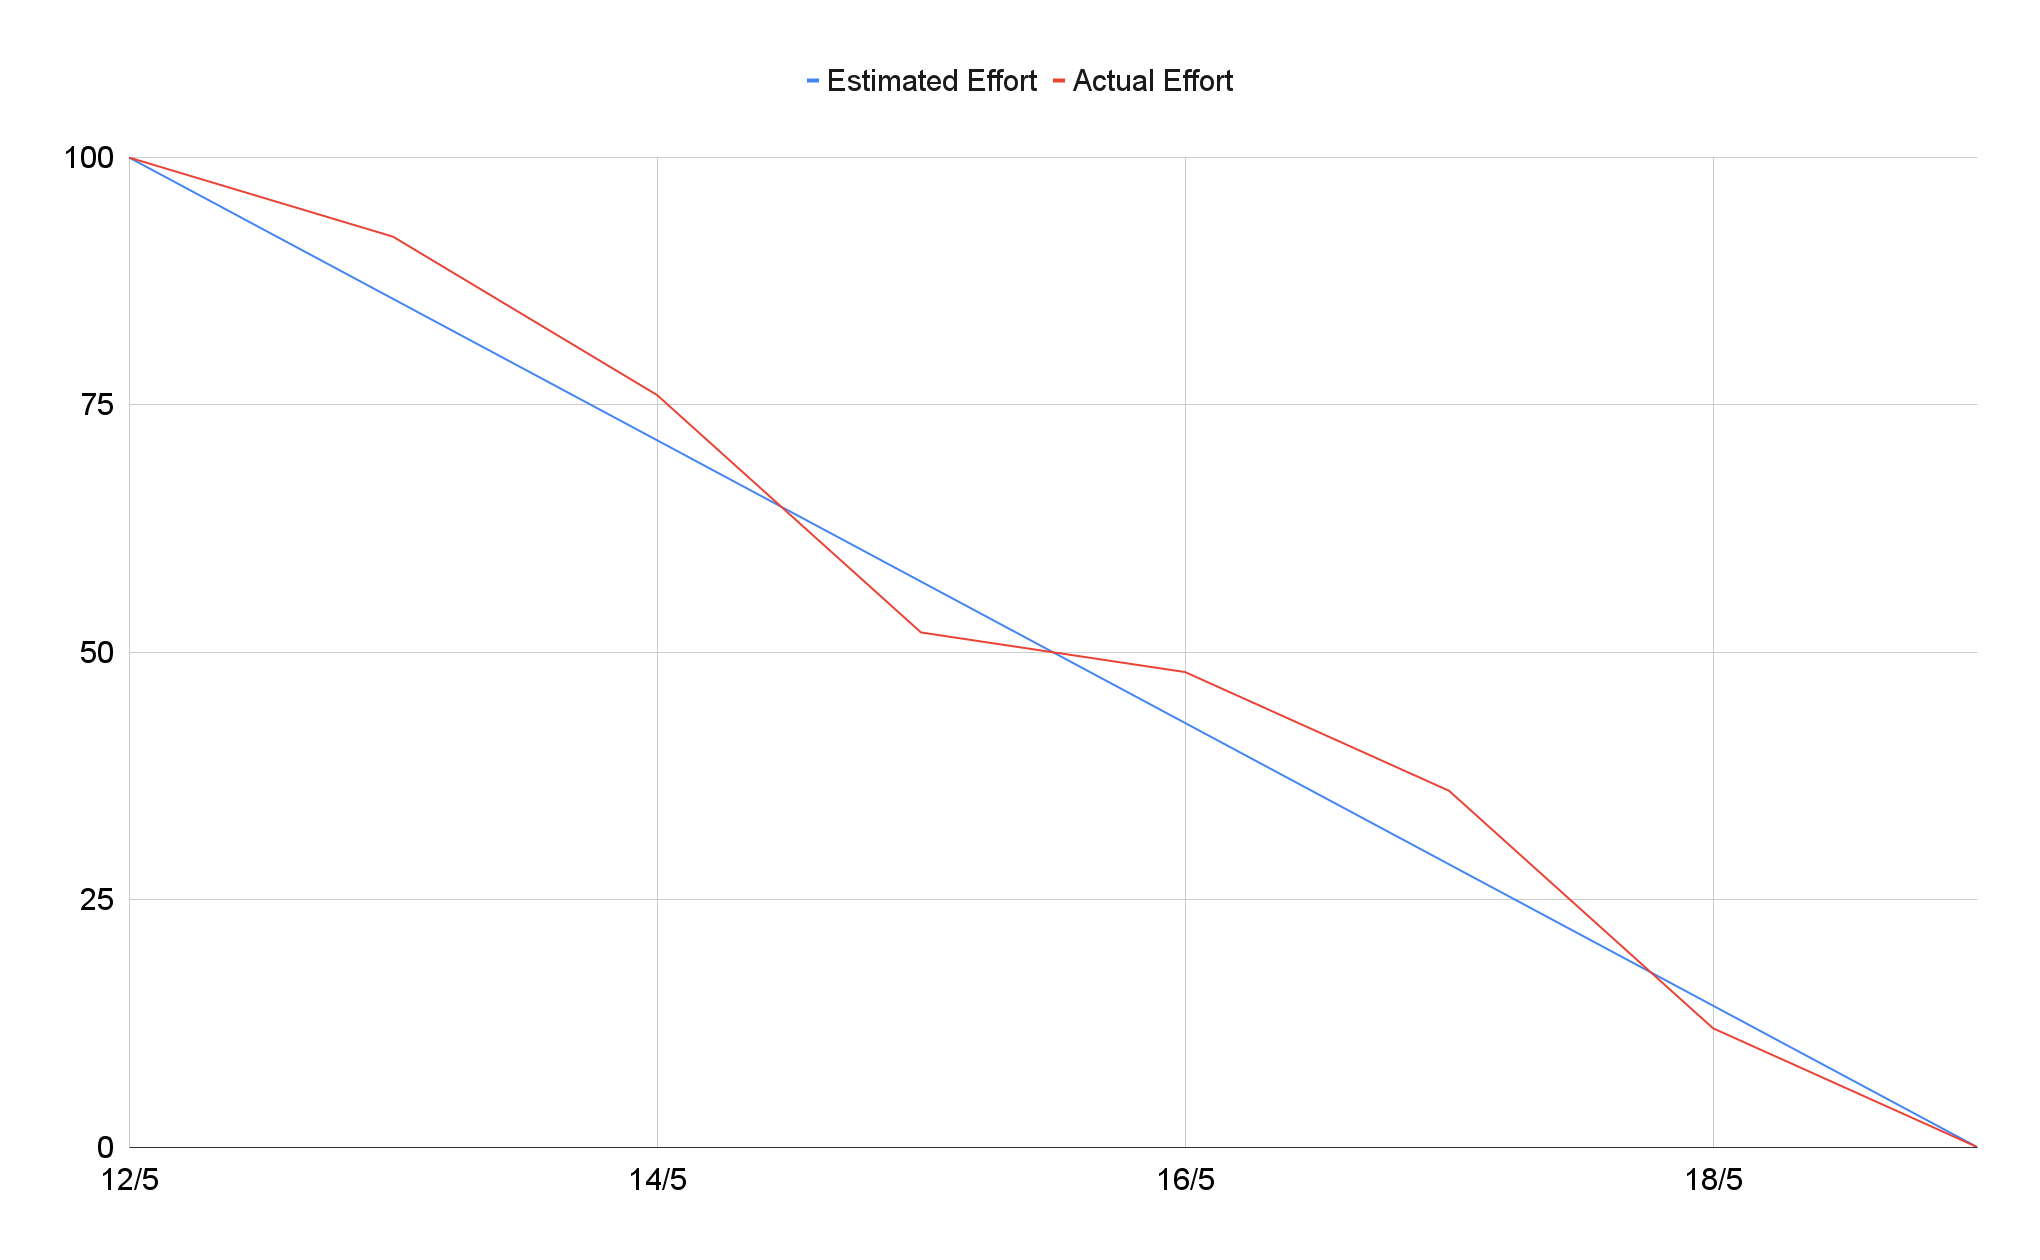
\includegraphics[width=0.95\textwidth]{images/burndown_chart.png}

\end{document}
